\section{Wikidata}

Wikidata is the free and open knowledge base created by the Wikimedia movement, which collects multilingual structured data in one central place and makes it publicly available under CC0, a ``Public Domain Dedication'' \citep{cc0}, and therefore free for anyone to copy, use and distribute. \\
In common with Wikipedia, it can be edited by anyone. Wikidata collects data on different topics such as people, places, events and many more in so called \textit{items}.
\begin{figure}[H]
	\centering
	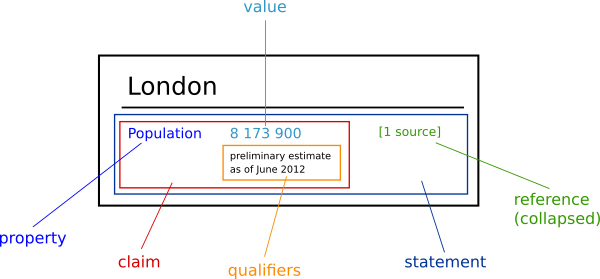
\includegraphics[width=\textwidth]{diagrams/Wikidata_statement.png}
	\caption{Example for Wikidata item \textit{``Douglas Adams'' (Q42)}, by \citet{kritschmar}}
	\label{diagramWikidataStatement}
\end{figure}
Every item has an identifier, starting with the letter ``Q'' followed by a unique number. It is therefore clearly identifiable and not depending on labels in natural language, which may change or be ambiguous. Additionally this offers the possibility of referring to the same item in multiple languages using only one ID. \\
Statements contain a \textit{property}, which is the core part and indicates, what kind of statement is made, and references to prove the claim. One or more values are attached to this property. For example, a claim for a city could be the property \textit{``Population'' (P1082)} with the respective number of inhabitants. There can be multiple values for population for different years, differentiated by \textit{qualifiers}. To identify the important and most recent data, the values can be marked as preferred, normal and deprecated. If the claim has references proving the facts stated, it's a statement. \\
Data types for the properties are \textit{item}, textit{string}, textit{quantity}, textit{name of Wikimedia Commons file}, textit{geo coordinate}, textit{time}, textit{URL}, and simultaneously developed to the ArticlePlaceholder extension are textit{mathematical expressions}, and textit{identifiers of other databases} such as VIAF. \\
Properties and items are called \textit{entities} in Wikidata. \\
Items can have \textit{sitelinks}. Sitelinks are links to Wikipedia or other Wikimedia projects such as Wikivoyage. \\
\\
The aim is to have a knowledge base that supports Wikipedia and can also be used in other contexts in the semantic web. Therefore Wikidata offers an API as well as a SPARQL endpoint. Additionally, the data can be downloaded as a full database dump in the formats JSON, XML and RDF. \todo[inline]{Wikidata's connection to Wikipedia}